\subsection*{Первая задача}


Зная состояние в $| l,\, l\rangle $
\begin{equation*}
    Y_{ll} = C_l e^{i l \varphi} \sin^l \theta, \hspace{5 mm} 
    c_l = \left[
        \frac{(-1)^l}{2^l l!}
    \right] \sqrt{\frac{(2l+1)(2l)!}{4\pi}},
\end{equation*}
с помощью понижающего оператора
\begin{equation*}
    \hat{L}_- = i \hbar e^{-i \varphi} \left(i \partial_\theta + \ctg \theta \partial_\varphi\right),
\end{equation*}
найдём состояния с $l=1$ и $m = -1, 0, +1$. Для начала,
\begin{equation*}
    Y_{11} = \left(\frac{-1}{2}\right) \sqrt{\frac{3 \cdot 2}{4 \pi}} e^{i \varphi} \sin \theta = - \frac{1}{2} \sqrt{\frac{3}{2\pi}} e^{i \varphi} \sin \theta.
\end{equation*}
Теперь вспомним, что
\begin{equation*}
    \hat{L}_- | l,m\rangle =  \sqrt{(l+m)(l-m+1)} \hbar | l,m\rangle,
    \hspace{5 mm} 
    \langle \theta, \varphi| \hat{L}_- | 1,1\rangle = \hbar \sqrt{2} \langle \theta, \varphi \,|\, 1,0 \rangle = \hat{L}_- \langle \theta,\varphi \,|\, 1,1 \rangle = \hat{L}_- Y_{11},
\end{equation*}
теперь, с учётом нормировки, подставляем $\hat{L}_-$ и находим
\begin{equation*}
    Y_{10} = \hat{L}_- \frac{Y_{11}}{\hbar \sqrt{2}} = 
    \frac{e^{-i \varphi}}{\sqrt{2}} \left(
        - \partial_\theta + i \ctg \theta \ \partial_\varphi
    \right) \left(
        - \tfrac{1}{2} \sqrt{\tfrac{3}{2\pi}} e^{i \varphi}\sin \theta
    \right) = \frac{1}{2} \sqrt{\frac{3}{\pi}} \cos \theta.
\end{equation*}
Аналогично повторяем операцию понижения,
\begin{equation*}
    Y_{1,-1} = \hat{L}_- \frac{Y_{10}}{\hbar \sqrt{2}} = 
    \frac{e^{-i\varphi}}{\sqrt{2}} \left(
        - \partial_\theta + i \ctg \theta \, \partial_\varphi
    \right) \left(
        \frac{1}{2} \sqrt{\frac{3}{\pi}} \cos \theta
    \right) = \frac{1}{2} \sqrt{\frac{3}{2\pi}} e^{- i \varphi} \sin \theta.
\end{equation*}
Вид орбиталей $Y Y\con$ приведен на рисунке. \vspace{-5mm}
\begin{figure}[h]
    \centering
    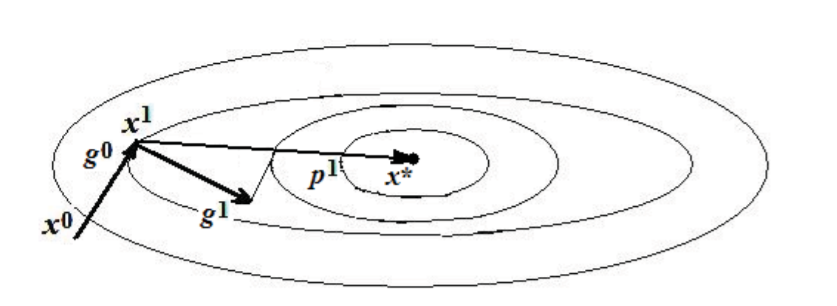
\includegraphics[width=0.7\textwidth]{D:\\Kami\\WM12_Workspace\\HydrogenOrbitals\\1.pdf}
    \caption{Вид орбиталей типа $Y_{1,1}$, $Y_{1,0}$, $Y_{1,-1}$.}
    %\label{fig:}
\end{figure}




\vspace{-10mm}
\subsection*{Вторая задача}


Хотелось бы найти $\bk{\theta, \varphi}[\hat{L}_y]{\alpha}$, для этого рассмотрим инфинитизимальное вращение на угол $\delta \xi$ вокруг оси $x$:
\begin{equation*}
    \bk{\vc{x}}[\mathbbm{1} - \tfrac{i}{\hbar} \delta \xi \hat{L}_y]{\alpha} = 
    \bk{x - z \delta \xi, y, z + x \delta \xi}{\alpha}.
\end{equation*}
Вспомним, что в сферических координатах
\begin{equation*}
    \left\{\begin{aligned}
        \delta x &= \cos \theta \cos \varphi \delta \theta- \sin \theta \sin \varphi \delta \varphi = - z \delta \xi \\
        \delta y &= \cos \theta \sin \varphi \delta \theta + \sin \theta \cos \varphi \delta \varphi = 0
    \end{aligned}\right.
    \hspace{0.5cm} \Rightarrow \hspace{0.5cm}
    \left\{\begin{aligned}
        \delta \theta &= - \cos \varphi \, \delta \xi \\
        \delta \varphi &= \ctg \theta \sin \varphi \, \delta \xi
    \end{aligned}\right.
\end{equation*}
Подставим это выражение в выражение для малой трансляции в сферических координатах:
\begin{equation*}
     \bk{\theta,\varphi}[\mathbbm{1} - \tfrac{i}{\hbar} \delta \xi \hat{L}_y]{\alpha} = 
     \bk{\theta,\varphi}{\alpha} + \partial_\theta (\bk{\theta, \varphi}{\alpha}) \delta \theta + \partial_\varphi (\bk{\theta, \varphi}) \delta \varphi,
\end{equation*}
где мы воспользовались аналитичностью. Тогда
\begin{equation*}
    \bk{\theta,\varphi}[\hat{L}_y]{\alpha} = i \hbar \left(
        - \cos \varphi \, \partial_\theta + \ctg \theta \sin \varphi \, \partial_\varphi
    \right) \bk{\theta,\varphi}{\alpha}, 
\end{equation*}
откуда и находим операторное равенство
\begin{equation*}
    \hat{L}_y = i \hbar \left(
        - \cos \varphi \, \partial_\theta + \ctg \theta \sin \varphi \, \partial_\varphi
    \right)
    , \hspace{5 mm} \text{Q. E. D.}
\end{equation*}